\documentclass[12pt]{article}

\usepackage{amsmath}
\usepackage{amssymb}
\usepackage{calc}
\usepackage{units}
\usepackage{graphicx}
\usepackage[pdftex]{hyperref}
\usepackage{subfig}
\usepackage[margin=1in]{geometry}
\usepackage{listings}
\usepackage[numbers,sort&compress]{natbib}
\usepackage{bm}
\usepackage{paralist}
\usepackage[draft]{fixme}
\usepackage{textcomp}
\usepackage{yorkdefs}

\newcommand{\halflife}{\ensuremath{T_{\nicefrac{1}{2}}}\xspace}

\hypersetup{
  breaklinks=true,
  pdftitle={Alternating Current RLC Circuits},
  pdfauthor={Kevin R. Lynch based on a lab by D.C.Jain}, 
  pdfsubject={Phyiscs, Electricity and magnetism},
  pdfkeywords={resistance, inductance, capacitance, alternating current},
  pdflang={en-US},
}

\title{Alternating Current RLC Circuits}
\author{}
%Kevin R. Lynch, based on an earlier lab by D.C.Jain
%\date{2012-03-23}
\date{}

\begin{document}

\maketitle

\section{Objectives}
\label{sec:objectives}

\begin{enumerate}
\item To understand the voltage/current phase behavior of RLC circuits
  under applied alternating current voltages,
\item To understand the current amplitude behavior of RLC circuits
  under applied alternating current voltages, and
\item To understand the phenomenon of resonance in RLC circuits.
\end{enumerate}

\section{Introduction}
\label{sec:introduction}

\begin{figure}
  \centering
  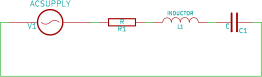
\includegraphics[width=2\textwidth/3]{figures/rlc-circuit}
  \caption{The RLC circuit.}
  \label{fig:rlccircuit}
\end{figure}
In previous labs\footnote{\textit{Alternating Current RC Circuits} and
  \textit{Alternating Current RL Circuits}} you studied the behavior
of the RC and RL circuits under alternating applied (or AC) voltages.
Here, you will study the behavior of a similar circuit containing
series connected capacitor, inductor, and resistor.  This is, quite
reasonably, called an \textit{RLC Circuit}; see
Figure~\ref{fig:rlccircuit}.

\section{Theory}
\label{sec:theory}

Once again, let's analyze this circuit using Kirchoff's Rules.  As
always, you find
\begin{gather*}
  V_s(t) - V_R(t) - V_L(t) - V_C(t) = 0\ ,
\end{gather*}
leading to a differential equation we have not encountered in these
labs before
\begin{gather*}
  \deriv[2]{q(t)}{t} + \frac{R}{L} \deriv{q(t)}{t} + \frac{1}{LC} q(t)
  = V_s(t)\ ,
\end{gather*}
where $q(t)$ is the charge on the capacitor.  We will not actually
solve this equation, as the derivation is beyond the mathematics level
of this course; however, in Appendix~\ref{sec:solutions} we quote some
important results.  For a sinusoidally varying source voltage
\begin{gather*}
  V_s(t) = V_s \cos\omega t\ ,
\end{gather*}
we find the current is again out of phase, but this time, whether the
current lags or leads the applied voltage depends on whether the
inductive or capacitive reactances (both defined as before) dominate
the behavior of the circuit at the driving voltage.  Comparing the
solutions in the Appendix with our differential equation here,
matching coefficients, we have
\begin{align*}
  \omega_0 &= \frac{1}{\sqrt{LC}} & 2\beta &= \frac{R}{L}\ .
\end{align*}
Putting all these definitions together, we can solve for the current
and voltage profiles as a function of frequency
\begin{gather*}
  I(t) = \frac{V_s \omega}{L} 
  \frac{\cos\left(\omega t + \delta\right)}
  {\sqrt{\left(\omega_0^2-\omega^2\right)^2 +
      \left(2\beta\omega\right)^2}}\\ 
  V_R(t) = I(t) R = V_s 2\beta\omega 
  \frac{\cos\left(\omega t + \delta\right)}
  {\sqrt{\left(\omega_0^2-\omega^2\right)^2 +
      \left(2\beta\omega\right)^2}}\\
  V_C(t) = q(t)/C = 
  V_s \omega_0^2 \frac{\sin\left(\omega t + \delta\right)}
  {\sqrt{\left(\omega_0^2-\omega^2\right)^2 +
      \left(2\beta\omega\right)^2}}\\ 
  V_L(t) = -L\deriv[2]{q(t)}{t} = 
  V_s \omega^2 \frac{\sin\left(\omega t + \delta\right)}
  {\sqrt{\left(\omega_0^2-\omega^2\right)^2 +
      \left(2\beta\omega\right)^2}}\\ 
\end{gather*}
where the phase is given by 
\begin{gather*}
  \tan \delta = \frac{\omega_0^2-\omega^2}{2\beta\omega}\ .
\end{gather*}

\begin{figure}
  \centering
  \subfloat[][90\textdegree Phase]{
    \includegraphics[width=\textwidth/3-0.1in]{figures/lissajous-90}
  }
  \subfloat[][45\textdegree Phase]{
    \includegraphics[width=\textwidth/3-0.1in]{figures/lissajous-45}
  }
  \subfloat[][1\textdegree Phase]{
    \includegraphics[width=\textwidth/3-0.1in]{figures/lissajous-1}
  }
  \caption{Three example plots for the XY mode of the oscilloscope.
    In each plot, I show $V_R(t)$ versus $V_s(t)$; the frequencies of
    the two signals are the same, while the amplitude of $V_R(t)$ is
    smaller than $V_s(t)$.  On the left, they are 90\textdegree out of
    phase; in the middle, 45\textdegree; on the right, they are one
    degree out of phase.}
  \label{fig:lissajous}
\end{figure}
One useful tool for the study of two equifrequency signals is the XY
mode of the oscilloscope.  In the standard mode of the oscilloscope,
you can think of the display as a standard plot of the signal, with
the independent variable, $t$, on the horizontal axis, and the
dependent variable, $V(t)$, on the vertical axis.  The XY mode can be
thought of as a parametric plot, where the independent variable, $t$,
is implicit (not displayed), while the horizontal and vertical axes
trace out two different dependent variables, $V_1(t)$ and $V_2(t)$.
The XY mode is most useful when the two signals have commensurate
frequencies (their ratio is rational), particularly when their
frequencies are the same.  In these cases, the XY signals give both
relative frequency and relative phase information in an easy to
interpret manner; such plots are called \textit{Lissajous
  Figures}. Figure~\ref{fig:lissajous} shows a few of these plots.
When the two signals have the same frequency, the figure traces an
ellipse.  The major axis of the ellipse rotates, and the minor axis
shrinks, as the phase changes.  As the phase approaches 0, the minor
axis also vanishes.

Just as in the RC and RL settings, we can define a circuit impedance
by
\begin{gather*}
  Z^2 = R^2 + \left(X_L-X_C\right)^2\ ,
\end{gather*}
which has all the same consequences for the relationships between the
voltage amplitudes as it did for the $RC$ and $RL$ circuits.  We could
rewrite this equation in terms of the voltage amplitudes (that's
mostly left to you; see the Pre-Lab exercises); here we'll only note
the phase.  You can show
\begin{gather*}
  \tan \delta = \frac{X_L - X_C}{R}\ .
\end{gather*}

\begin{figure}
  \centering
  \subfloat[][Phases]{
    \includegraphics[width=\textwidth/2-0.1in]{figures/frequency-phase}
  }
  \subfloat[][Resistor voltage amplitude]{
    \includegraphics[width=\textwidth/2-0.1in]{figures/frequency-amplitudes}
  }\\
  \subfloat[][Capacitor voltage amplitude]{
    \includegraphics[width=\textwidth/2-0.1in]{figures/frequency-cap}
  }
  \subfloat[][Inductor voltage amplitude]{
    \includegraphics[width=\textwidth/2-0.1in]{figures/frequency-ind}
  }
  \caption{The phase angle as a function of angular frequency is on
    the upper left.  The resistor voltage/current amplitudes are
    displayed on the upper right.  The lower left shows the capacitor
    voltage amplitude, while the lower right shows the inductor
    voltage amplitude.  In all cases, the frequency is normalized in
    units of $\omega_0 = 1/\sqrt{LC}$.  Because the phase and
    amplitudes are also a function of $2\beta = R/L$, we plot families
    of curves for various values of $2\beta/\omega_0$.  The phase is
    normalized to $\pi/2$, while the amplitudes are normalized to
    $V_s$.}
  \label{fig:frequency}
\end{figure}
Just as we did for the RC and RL circuits, we should consider the
behavior of the RLC circuit as a function of frequency \ldots and
we're in for some new surprises, with very rich and interesting
phenomenology. Consider first the phase.  Notice that $\delta=0$ when
$X_L = X_C$.  This is called the \textit{phase resonance} of the
circuit.  At what frequency, $\omega_R$, does this happen?
\begin{gather*}
  X_L = X_C = \omega_R L = \frac{1}{\omega_R C} \longrightarrow
  \omega_R = \frac{1}{\sqrt{LC}} = \omega_0\ .
\end{gather*}
This is called the \textit{natural} frequency of the circuit.  Where
$X_L$ dominates $X_C$, the current lags the drive voltages, while the
current leads the drive voltage in the opposite case.  Thus, the phase
can vary between $-\pi/2$ and $\pi/2$, depending on the values of the
circuit components.

There are a number of other resonances for this circuit.  We can, for
instance, look for the maxima of the voltage amplitudes, the so called
\textit{amplitude resonances} of the circuit; see
Figure~\ref{fig:frequency}.  To predict these, we extremize the
amplitudes versus the frequencies ($\deriv{A(\omega)}{\omega} = 0$).
Clearly the current and the voltage across the resistor will be
maximized at the same frequency:
\begin{gather*}
  \left.\deriv{V_R(\omega)}{\omega}\right|_{\omega_R} = 0
  \longrightarrow \omega_R = \omega_0\ ,
\end{gather*}
or the \textit{current amplitude resonance} occurs at the same
frequency as the natural oscillation frequency of the circuit.
Interestingly, the amplitude resonance for the capacitor and inductor
voltages are \textit{not} the same as for the current!  For the
capacitor,
\begin{gather*}
  \left.\deriv{V_C(\omega)}{\omega}\right|_{\omega_C} = 0 
  \longrightarrow \omega_C = \sqrt{\omega_0^2 -
      \nicefrac{1}{2}(2\beta)^2}\ ,
\end{gather*}
the resonant voltage amplitude across the capacitor occurs at a
\textit{lower} frequency than the phase resonance!  For the inductor,
\begin{gather*}
  \left.\deriv{V_L(\omega)}{\omega}\right|_{\omega_L} = 0 
  \longrightarrow \omega_L = \sqrt{
      \frac{\omega_0^4}{\omega_0^2 - \nicefrac{1}{2}(2\beta)^2}
    }\ .
\end{gather*}
the resonant voltage amplitude occurs at a frequency \textit{higher}
than the phase resonance.  Of course, these last two resonance
conditions will only occur if the radical is real.

\section{Procedures}
\label{sec:procedures}

You should receive two multimeters (one of which should be a
BK-5460), an oscilloscope, a function generator, a
decade resistance box, a decade capacitance box, and an inductor.

\begin{enumerate}
\item First, select component values for testing.  Select a frequency
  between \unit[300]{Hz} and \unit[600]{Hz}, and a value for $C$
  between $\unit[0.06]{\mu F}$ and $\unit[0.1]{\mu F}$.  Record the
  value of the inductance, $L$.  Measure and record the values of the
  inductor resistance $R'$, and $C$.  Calculate $X = \left| X_L-X_C
  \right|$ and choose a value for $R + R' \approx 1.2 X$.  Set,
  measure and record $R$.
\item Configure the circuit for testing shown in
  Figure~\ref{fig:rlccircuit}.  Insert the Simpson multimeter to
  record the AC current.
\item Using the BK Precision meter, record the frequency $f$, and the
  RMS AC voltages across the signal generator $V_s$, the resistor
  $V_R$, the capacitor $V_C$, and the inductor $V_L$.  Are these
  values consistent?
\item \label{item:phase} Measure the phase shift between the current
  and applied voltage for your chosen frequency.  Connect the
  oscilloscope so as to measure the voltage across the resistor and
  signal generator; make sure the negtive inputs share a common
  reference point.  Make sure the two signal baselines are centered
  with respect to the horizontal and vertical axes of the
  oscilloscope, and adjust the voltage and time scales so that
  slightly more than one cycle of both waveforms is visible.  Measure
  the phase shift as you did in the previous lab.  Increase the
  frequency by 50\%, and determine the phase shift again.  Halve the
  initial frequency, and repeat.
\item \label{item:phase_resonance} Next, find the resonant frequency.
  First, predict the value.  Then, go searching for it experimentally.
  There are three methods to do this:
  \begin{enumerate}
  \item Find the frequency which maximizes the current (or the voltage
    across the resistor), 
  \item Find the frequency which eliminates the phase shift in AB
    mode, or
  \item Find the frequency which collapses the XY mode Lissajous
    figure to a line.
  \end{enumerate}
  In an ideal world each method should give the same result, although
  the last method is both easiest and most accurate.  Do all three
  methods, in fact, produce the same result?
\item \label{item:current_response} Next, map out the amplitude of the
  current response.  Without changing $R$ or $C$, vary the frequency
  over, say, ten points, and record the frequency, RMS voltage $V_s$
  and RMS current $I$ at those points.  The low frequency should be
  about half the phase resonance, the high frequency should be about
  twice the phase resonance, and the middle point should be at the
  phase resonance.
\item \label{item:amplitude_resonance} Finally, let's search for the
  amplitude resonances of $V_C(t)$ and $V_L(t)$.  Without changing
  $C$, set $R+R'=0.4X$.\footnote{Why do we have to change $R$?}
  Confirm that the phase resonance has the same frequency.  Predict
  the frequencies of both amplitude resonances.  Using either the
  multimeter or the oscilloscope, search for the amplitude resonances.
  Do they match your prediction?
\end{enumerate}

\appendix

\section{Derivation of Solutions}
\label{sec:solutions}

Applying Kirchoff's rules to the series RLC circuit leads to a second
order linear differential equation with constant coefficients, with a
driving function.  We won't solve this function in all its glory as we
did for the first order equation that arises for the RC and RL
equations.  In fact, solving the equation is somewhat beyond the level
of the prerequisite mathematics for this course, so we'll just quote
the solution here.\footnote{Although you can look up the solution
  methods on the net, or in any standard sophomore level physics or
  mathematics text.  I take the notation from Marion and Thornton's
  \textit{Classical Dynamics}.}

Let's write the differential equation in the form
\begin{gather*}
  \deriv[2]{q(t)}{t} + 2 \beta \deriv{q(t)}{t} + \omega_0^2 q(t) = A
  \cos\omega t\ .
\end{gather*}
A full solution to this equation can be written in terms of two
functions: 
 \begin{enumerate}
\item The ``complementary'' or ``homogeneous'' solution $q_c(t)$, when
  $A=0$.  This is the transient solution, and decays away
  exponentially; we'll not dwell on this any further.
\item The ``particular'' solution $q_p(t)$, where we don't drop the
  driving term.  We previously called this one the ``steady state''
  solution.  Typically, we take ``trial solutions'' of the same form
  as the driving term, and see if we can come work up a function that
  satisfies the equation.
\end{enumerate}
Let's try a particular solution that's a sinusoid.  Before diving in,
let's think about the \textit{form} of the physical solution that
we're looking for here.  In our specific problem, the solution to the
differential equation is the charge on the capacitor, but the physics
we're interested in is the phase difference between the
\textit{current} and the drive voltage.  Thus, we want a current that
is of the same functional form as the drive voltage, plus a phase
offset.  Since we choose a drive voltage that is a cosine, and current
is the derivative of the charge, we want to choose a steady state
(particular) solution of the form
\begin{gather*}
  q_p(t) = D \sin\left( \omega t + \delta \right)\ .
\end{gather*}
To show this is a solution, we need to find $D$ and $\delta$, which we
do by substituting into the differential equation, to obtain
\begin{gather*}
  -D\omega^2 \sin\left(\omega t + \delta\right) + 2\beta D\omega
  \cos\left(\omega t + \delta\right) + D\omega_0^2 \sin\left(\omega t
    + \delta\right) = A \cos\omega t\ .
\end{gather*}
Next, we expand the $\sin$ and $\cos$ terms, since:
\begin{align*}
  \cos(a+b) &= \cos\omega t \cos\delta - \sin\omega t \sin\delta &
  \sin(a+b) &= \sin\omega t \cos\delta + \cos\omega t \sin\delta\ ,
\end{align*}
which gives six terms on the left, half of which contain a $\sin\omega
t$ and the other have contain $\cos\omega t$.  The right hand side
contains only $\cos\omega t$.  If this is a solution, the coefficients
of the $\sin\omega t$ and $\cos\omega t$ terms must separately be
equal, and must be collectively consistent.  Thus, we have two
equations for the two unknowns $D$ and $\delta$
\begin{gather*}
  \sin\omega t: \qquad -D\omega^2 \cos\delta - 2\beta D\omega
  \sin\delta + D\omega_0^2 \cos\delta = 0\\
  \cos\omega t: \qquad -D\omega^2 \sin\delta + 2\beta D\omega
  \cos\delta + D\omega_0^2 \sin\delta = A\ .
\end{gather*}
The $\sin\omega t$ equation can be solved for $\delta$
\begin{gather*}
  \tan\delta = \frac{\omega_0^2 - \omega^2}{2\beta\omega}\ .
\end{gather*}
Now that we have $\delta$, we can use the second equation to solve for
$D$
\begin{gather*}
  D = \frac{A}{\left(\omega_0^2-\omega^2\right) \sin\delta +
    2\beta\omega \cos\delta}\ .
\end{gather*}
How do we substitute for $\delta$ in this latter equation?  Using the
trigonometric relations
\begin{align*}
  \tan\delta &= \frac{\sin\delta}{\cos\delta} & 
  \sin^2\delta + \cos^2 \delta &= 1\ ,
\end{align*}
you can show that
\begin{align*}
  \sin\delta &= \frac{\omega_0^2 -
    \omega^2}{\sqrt{\left(\omega_0^2-\omega^2\right)^2 +
      \left(2\beta\omega\right)^2}} & 
  \cos\delta &=
  \frac{2\beta\omega}{\sqrt{\left(\omega_0^2-\omega^2\right)^2 + 
      \left(2\beta\omega\right)^2}}\ .
\end{align*}
Substituting these values, you will obtain the coefficient $D$
\begin{gather*}
  D = \frac{A}{\sqrt{\left(\omega_0^2-\omega^2\right)^2 + 
      \left(2\beta\omega\right)^2}}\ .
\end{gather*}


\newpage
 
\section*{Pre-Lab Exercises}

Answer these questions as instructed on Blackboard; make sure to
submit them before your lab session!

\begin{enumerate}
\item Derive a relationship between the voltage amplitudes $V_s$,
  $V_R$, $V_C$, and $V_L$ for the RLC circuit.  Hint: how is $V_s$
  related to the impedance?
% V_s^2 = V_R^2 + (V_L-V_C)^2
\item A series RLC circuit is driven at \unit[500]{Hz} by a sine wave
  generator.  It has parameters $R=\unit[5]{k\Omega}$, $L =
  \unit[2]{H}$, and $C = \unit[2]{\mu F}$.  What is the impedance of
  the circuit?
% 7.9kOhm
\item What is the phase resonance frequency for the circuit in the
  previous question?
% 79.5Hz
\item Does this circuit have amplitude resonances?  If so, what are
  their frequencies?
% no
\item If you use instead a $\unit[0.08]{\mu F}$ capacitor, does the
  circuit have amplitude resonances?  If so, what are their
  frequencies?  What is the new phase resonance?
% yes, 397Hz, 281Hz, 563Hz
\end{enumerate}

\newpage

\section*{Post-Lab Exercises}

\begin{enumerate}
\item From your recorded inductance, and the measured resistance,
  capacitance, inductance, and initial frequency, determine the
  impedance of your circuit.  Make sure to estimate your
  uncertainties.  Determine the impedance experimentally via another
  method, taking care of the uncertaintites. % V_s/I
  Do you get the same results?
\item Estimate the uncertainties on the measured values of $V_s$,
  $V_L$, $V_C$, and $V_R$.  Are these values consistent with each
  other?  Explain what you mean by ``consistent''.
\item From your measurements in Step~\ref{item:phase} of the
  procedure, determine the phase shift at each of the three measured
  frequencies, including an estimate of the uncertainty.  How do these
  compare to the theoretical predictions? 
\item Are your three measurements of the phase resonance frequency in
  Step~\ref{item:phase_resonance} consistent with each other?  With
  theoretical prediction?
\item Describe qualitatively what happens to your signals when you
  vary the frequency around the phase resonance.
\item Is your data from Step~\ref{item:current_response} consistent
  with the predictions of theory?  Specifically, do the voltage and
  current amplitudes measured by oscilloscope and by multimeter match,
  within uncertainties, and do they comport with theoretical
  expectations?
\item Why did you have to change the resistance value for
  Step~\ref{item:amplitude_resonance}?  Did you find the amplitude
  resonances?  If so, do their values agree with your theoretical
  predictions?
\item Discuss briefly whether you have met the objectives of the lab
  exercises.
\end{enumerate}

\end{document}

%%% Local Variables: 
%%% mode: latex
%%% TeX-master: t
%%% End: 
